% !TeX root = ../main.tex

\chapter{简介}
    随着线上教育模式的快速发展与普及,互联网上有越来越多的教育视频可供人们学习。
    面对海量的教育类视频,一个自动化的教育视频知识点预测系统能够快速有效地帮助人们识别视频中涉及的知识,使人们能够更轻松地从中找到符合自身正在学习的知识点的视频,从而大大减少人们寻找学习视频的成本。
    教育视频的知识点预测也是许多针对视频的下游任务的基础,比如相似知识点视频推荐、视频推题任务等。

    \begin{figure}[t]
        \centering
        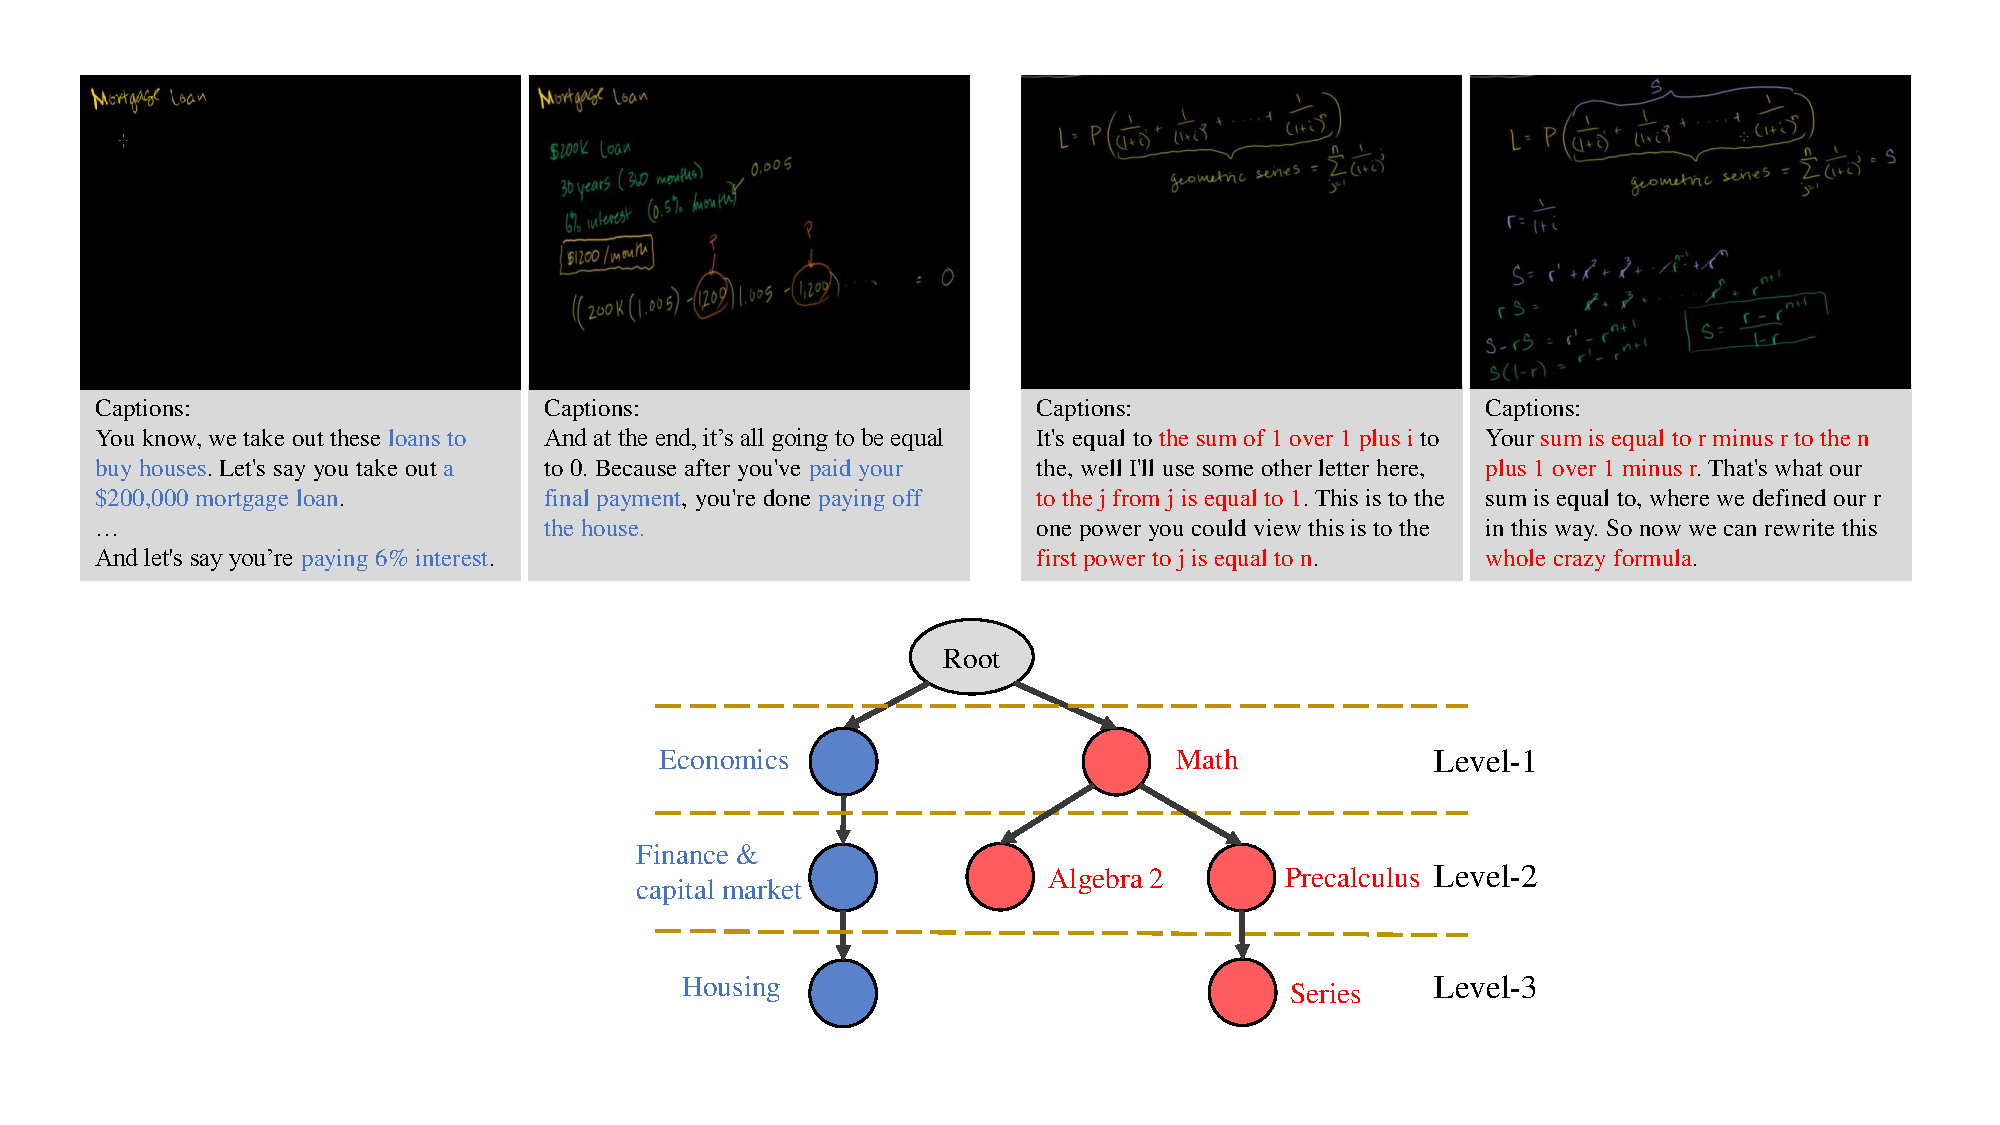
\includegraphics[width=1\linewidth]{data-example.pdf}
        \caption{教育类视频及知识点示例}
        \label{fig1.1}
    \end{figure}

    图 \ref{fig1.1} 中给出了一个教育类视频的示例。可以看出,教育类视频至少有着字幕文本、视频图像这两种模态的信息,
    如何有效地将视频中多种模态的信息进行提取与融合对于教育类视频的知识点预测而言是一个重要的问题。
    同时,教育类视频也有着显著的分块讲解的特点,图 \ref{fig1.1} 中前两张视频帧和后两张视频帧的内容之间存在着较大的差异。
    我们分别使用蓝色和红色对字幕文本中涉及经济学、数学的关键词进行标记,前两帧之间的视频主要在讲授经济学的内容,而后两帧之间的视频主要在讲授经济学现象背后的数学原理与计算方法。
    我们在图 \ref{fig1.1} 的右侧给出了该视频涉及的知识点标签。同样地,我们分别用蓝色与红色标记和经济学、数学相关的知识点标签。
    我们可以看到知识点标签之间存在着层级的关系,在这个知识点层级结构中,越上层的知识点越宽泛、抽象,越下层的知识点越细致、具体。
    一个教育类视频通常会包含知识点体系中多个属于不同层级的知识点,对教育类视频进行知识点预测,还需要考虑到知识点之间的层级关系。
    因此,教育类视频的知识点预测任务本质上是一个包含多模态信息的\textbf{层级多标签分类}(Hierarchical Multilabel Classification, HMC)任务。

    \textbf{多模态数据中所包含的信息是非常丰富的},人天生具有同时接收多种模态信息的能力,并能够将它们进行内在的关联,从而挖掘出更多隐含的信息,而这对于计算机而言绝非易事。
    在多模态机器学习领域中,使用多模态数据进行各种任务之前,首先需要对多模态数据中包含的信息进行表征。
    为了提取图像中的特征信息,研究人员先后提出多种神经网络方法,包括卷积神经网络\cite{Krizhevsky2012ImageNetCW}、3D卷积神经网络\cite{Tran2015LearningSF}、残差网络\cite{He2016DeepRL}等,这些神经网络方法通过研究图像中局部像素之间的关联来达到提取特征的目的。
    对于文本信息而言,基于循环神经网络的 LSTM\cite{Hochreiter1997LongSM} 通过序列学习的方式提取文本中隐含的信息,
    近年也有基于注意力机制的大型深度网络 BERT\cite{Devlin2019BERTPO} 来对文本进行特征提取。
    \textbf{总而言之,一个有效的多模态特征表示对于多模态机器学习而言是至关重要的}\cite{Baltruaitis2019MultimodalML}。
    多模态的数据中所包含的信息通常不仅仅是各个单独模态信息的简单相加,也包括各模态信息之间互相关联而产生的关联信息。
    比如在一段教育类视频中,通过结合视频与字幕文本两种模态信息,我们可以得到教师整堂课讲授的重点区域的内容。 
    因此在得到多模态数据各个模态信息的特征表示之后,\textbf{对多模态特征进行特征融合也很重要。}
    多模态特征融合不仅能提取出各模态信息之间的关联信息,同时还能提高各模态信息中共同部分的特征表示的鲁棒性\cite{Baltruaitis2019MultimodalML},\textbf{这在某些模态信息存在噪声时能有着更好的抗噪能力}。
    % 多模态特征融合根据融合的时机可以分为三种模式:Early、Late 和 Hybrid。
    % Early 模式的特征融合表现为在完成多模态特征抽取之后直接就将特征表示进行融合,然后再将融合特征应用于下游任务。
    % Late 模式的特征融合表现为分别使用各个模态的特征表示完成下游任务,最后再将各个模态得到的结果进行综合。
    % Hybrid 模式即为 Early 模式和 Late 模式的综合。
    对于教育视频的知识点预测而言,因为教育视频主要包含的模态信息为视频与字幕文本,因此如何有效地对这两种模态信息进行特征表示,以及如何有效地将这两种模态的特征进行融合将是我们需要解决的问题。

    相比于普通的多标签分类任务,层级多标签分类任务的特殊性在于标签之间存在内在关联。
    层级标签体系通常被组织成多叉树或是有向图的形式,不同层级的标签之间需要满足\textbf{真实路径规则}(True Path Rule, TPR)\cite{Valentini2009TruePR}。
    真实路径规则的含义为,在一个层级标签体系中,若一个标签被标记为正,则所有该标签的祖先标签都需要被标记为正;相反地,若一个标签被标记为负,则所有该标签的子标签都应该被标记为负。
    自层级多标签分类任务产生以来,已经有许多流派的工作为这个领域作出了贡献。
    首先是最简单的平坦化分类方式,这种分类算法通过只对最后一层标签\cite{Barbedo2007AutomaticGC}进行预测的方式,将层级多标签分类任务转化为了普通的多标签分类任务。
    平坦化分类方式隐含地使用了 TPR,即若最后一层中有标签被预测为正,则自动地将所有该标签的祖先标签都标记为正。
    这种分类方法虽然实现简单且不会违背 TPR,但是它忽略了层级标签体系内部的内在关联,也失去了标签体系中包含的信息。
    为了解决平坦化分类方式存在的问题,后续有工作开始尝试利用标签层级体系进行局部分类。
    这种局部分类的方式还可以细分为三种形式,第一种是对层级标签体系中的每一个标签都训练一个分类器(Local Classifier per Node, LCN)\cite{CesaBianchi2004IncrementalAF},用于对该标签进行二分类;
    第二种是在所有具有子标签的标签上训练一个分类器(Local Classifier per Parent Node, LCPN)\cite{Secker2007AnEC},用于对该标签的的子标签进行分类;
    最后一种是对层级标签体系中的每一层标签训练一个分类器(Local Classifier per Level, LCL)\cite{Freitas2007ATO},用于对下一层标签进行分类。
    因为这两种分类方式在分类器分类时都只考虑到了层级标签体系中的一部分,因此称为局部分类。
    局部分类相较于平坦化分类考虑到了层级体系中所有的标签,而不仅仅是最后一层标签,同时也将不同层标签之间的关联进行了建模,因此较平坦化分类方式有着更好的分类性能。
    但是局部分类方式可能会面临层级不一致的问题,即分类结果可能不满足 TPR。

    因此,对教育类视频进行知识点预测存在着以下三个问题:
    首先是教育类视频的信息密度较大,且视频时长通常较长,比如在我们实验的数据集中视频的平均长度在 7 分钟以上。若直接将整个视频输入到知识点预测模型中,可能会造成模型对视频多模态信息利用率不佳。
    因此需要选择一个合适的视频切分方式,将教育类视频分块进行预测,最后再对结果进行综合,以充分地利用视频中的所有多模态信息。
    其次是对教育类视频的多模态特征表示和特征融合。多模态融合特征将用于层级知识点的预测,因此在多模态特征提取与融合阶段得到的特征向量质量的优劣,将会对后续知识点预测的性能造成直接影响。
    最后是在对层级知识点进行预测时,如何结合平坦化分类方式与局部分类方式,使得知识点预测模型既具有局部分类方式的较高性能,又尽量不违背 TPR。

    为了解决以上三个问题,我们使用了一种\textbf{多模态的知识点预测网络(Multi-modal Knowledge Prediction Network, MKPN)}。
    具体而言,首先我们对输入的教育类视频根据视频讲解内容进行关键帧抽取并切分,得到一系列视频块与相应的字幕文本段。
    然后对于每一段视频块和字幕文本,我们分别使用残差网络和双向 LSTM 来提取出视频块和文本段中的多模态信息。
    接着我们将视频和文本多模态信息输入到基于注意力机制的循环神经网络中进行特征融合,得到带有知识点信息的统一特征表示,同时结合层级知识点体系中的知识点特征信息对每一层的知识点进行局部预测。
    得到每一层知识点的统一特征表示与局部预测结果之后,我们将这些结果输入到混合预测模块中,计算出该视频块最终预测的知识点。
    最后,我们综合所有视频块的预测结果,就得到了原教育类视频所涉及到的知识点。

    我们在一个真实的教育数据集(Khan)上进行了知识点预测的性能实验,实验的最终结果也证明了我们所使用方法的有效性。

% \section{一级节标题}

% \subsection{二级节标题}

% \subsubsection{三级节标题}

% \paragraph{四级节标题}

% \subparagraph{五级节标题}
